\documentclass[11pt]{article}
\usepackage[margin=.8in,letterpaper]{geometry}
\usepackage{amsmath}
\usepackage{newtxtext,newtxmath}
\usepackage{cancel}
%%\usepackage{times}
\usepackage{siunitx}
\usepackage{enumitem}
%\usepackage{graphicx}
\usepackage{tikz}
%%\usepackage{mathpazo}
%%\usepackage{xcolor,colortbl}
%%\usepackage{hyperref}
%\usepackage{wrapfig}
%\usepackage{authblk}
%
%%\newcommand\vertarrowbox[2]{%
%%    \begin{array}[t]{@{}c@{}} #1 \\
%%    \rotatebox{90}{$\xrightarrow{\hphantom{abcdefgh}}$} \\[-1ex]
%%    \mathclap{\scriptstyle\text{#2}}%
%%    \end{array}}
%
%\setlength{\parindent}{0pt}
%\setlength{\parskip}{8pt}
%
%
\usetikzlibrary{decorations.pathmorphing,patterns}

\tikzset{
  >=latex,
}
\sisetup{
%  detect-all,
  per-mode=symbol
}

\title{AP Physics 2 Class 2: First Law of Thermodynamics}
\author{Dr.\ Timothy Leung\\Meritus Academy}
\date{Revised: \today}


\begin{document}
\maketitle

\section{Law of Conservation of Energy}
The first law of thermodynamics is the application of the law of conservation
of energy applied to a thermodynamic system. Beginning with the form that should
be most familiar to most students, the law of conservation of energy states that
the change energy $\Delta E_\text{sys}$ in a system is equal to the external work
$W_\text{ext}$ done \emph{to} the system.
\begin{equation}
  \boxed{ \Delta E_\text{sys} = W_\text{ext}}
  \label{conservation1}
\end{equation}
In most cases studied in introductory physics, the total system energy is called
the \textbf{mechanical energy}, which is the sum of
the kinetic energies and all potential energies, and Eq.~\ref{conservation1}
expands to
\begin{equation}
  \boxed{ \Delta K + \sum_i\Delta U_i = W_\text{ext}}
  \label{conservation2}
\end{equation}
For a \textbf{closed system} that is isolated from its surrounding, and
therefore does not interact with the surrounding, there is no external work
($W_\text{ext}=0$) and the total energy of the system remains constant, i.e.:
\begin{equation}
  \Delta K + \sum_i\Delta U_i = 0\quad\text{(closed system)}
  \label{isolate1}
\end{equation}
This gives the often-repeated statement that \emph{law of conservation of
  energy states that energy can neither be created nor destroyed; it can only
  changes in form.} This statement is, of course, perfectly adaquate for a
clsoed system, but the actual law of conservation of energy is more nuanced.

\subsection{Example of a Closed System: Vertical Spring-Mass}
Closed systems are discussed in other handouts in the course, but the
vertical spring-mass system perfectly summarizes a closed system. The system
consists of a mass, the spring and the Earth. As such, the total energy of this
system consists of:
\begin{itemize}[nosep]
\item The kinetic energy $K$ of the mass
\item The potential energy $U_e$ stored in the spring, and
\item The gravitational potential energy $U_g$ stored between the mass and the
  Earth
\end{itemize}
In this case, there are only two forces doing work: the spring force $\vec F_e$
and the gravitational force $m\vec g$. Both forces are conservative, and act
within the sytem, therefore, the system is closed, and the total energy is
conserved:
\begin{equation}
  K + U_g + U_e=\text{constant}
\end{equation}
Without other external forces, the spring-mass system will continue to oscillate
forever.

\section{Internal Energy}
Suppose, however, instead of a block of mass that is oscillating, we have a
container full of gas of a certain temperature $T$, as shown in Figure~\ref{vertical}.
\begin{figure}[ht]
  \centering
  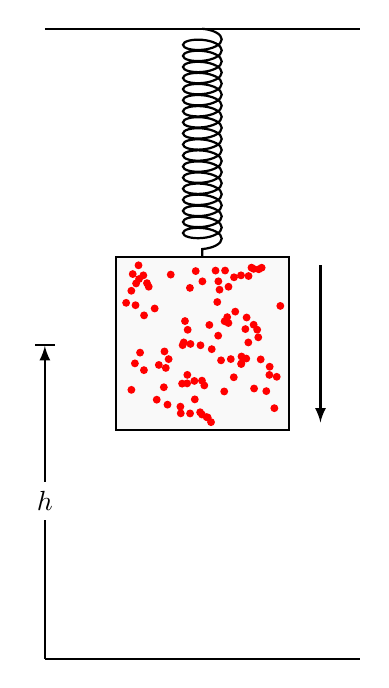
\begin{tikzpicture}
       \begin{scope}[thick]
        \draw(-1,5)--(3,5);
        \draw(-1,-3)--(3,-3);
        \draw[decoration={aspect=.4, segment length=4, amplitude=7, coil},
          decorate] (1,5)--(1,2.1); 
        \draw[fill=gray!5](-.1,-.1) rectangle(2.1,2.1);
        \draw[->](2.5,2)--(2.5,0) node[below]{$\varv$};
        \draw[|<-](-1,1)--(-1,-3) node[midway,fill=white]{$h$};
      \end{scope}
      \foreach \i in {1,...,90} \fill[red](rand+1,rand+1) circle(.05);
    \end{tikzpicture}
  \caption{A vertical spring-mass system with a container of gases.}
  \label{vertical}
\end{figure}
 The
gas molecules inside the container are all in random motion, and each of them
will have a kinetic energy. Therefore the conservation of energy must also
include the kinetic energies of \emph{all} the particles, as well as any undetermined
potential energies at the microscopic level, called the
\textbf{internal energy}, or \textbf{thermal energy}:
\begin{equation}
  U_\text{int} = K_\text{micro} + U_\text{micro}
\end{equation}
and the law of conservation of energy from Equation~\ref{conservation2} now
further expands to:
\begin{equation}
  \boxed{ \Delta K + \sum_i\Delta U_i + U_\text{int}= W_\text{ext}}
  \label{conservation3}
\end{equation}
For a monatomic or ideal gas, the internal energy consists only of the
transtional kinetic energies of the molecules, and therefore
\begin{equation}
  U=\frac32Nk_BT=\frac32nRT
\end{equation}
For diatomic gasses, the internal energy consists of the translational and
rotational kinetic energies:
\begin{equation}
  U=\frac52Nk_BT=\frac52nRT
\end{equation}
For solids, the internal energy consists of the translational energies and
spring potential energies when they are vibrating:
\begin{equation}
  U\approx3Nk_BT=3nRT
  \label{eq:solidU}
\end{equation}



\subsection{Equipartition Theorem}

\section{First Law of Thermodynamics}
Beginning with Equation~\ref{conservation3}, there are no changes in the bulk
kinetic energy and the potential energies:
\begin{equation}
  \xcancel{\Delta K} + \xcancel{\sum_i\Delta U_i} + U_\text{int}=
  W_\text{ext}
\end{equation}
But we must also consider the non-mechanical transfer of energy, called
\textbf{heat} $Q$, through conduction, convection and radiation. And finally
we arrive at the equation for the first law of thermodynamics:
\begin{equation}
  \boxed{ U = Q + W }
\end{equation}
As per tradition, we have dropped the ``int'' subscript for internal energy,
and the ``ext'' subscript for external mechanical work.


\section{Heat Capacity}
The \textbf{heat capacity} $C$ of an object directly relates the heat $Q$
transferred to the change in temperature, i.e.:
%heat needed to raise its temperature by \SI{1}{\kelvin}, i.e.:
\begin{equation}
  Q = C\Delta T
  \label{eq:heat-capacity}
\end{equation}
where hear $Q$ is measured in joules, and the change in temperature $\Delta T$
can be measured in either kelvin or degree Celsius. Heat capacity has a unit of
joule per kelvin (\si{\joule\per\kelvin}) or joule per degree Celsius
(\si{\joule\per\celsius}). Of course, this depends on \emph{what substance} the
objects is made of, and \emph{how much} of the sustance (i.e.\ its mass) there
is in the object. Therefore, a better quantity to use are the
\textbf{molar heat capacity} (heat capacity per mole of atoms):
\begin{equation}
  C_m=\frac Cn
\end{equation}
and the \textbf{specific heat capacity} (heat capacity per unit mass) $c$
\footnote{Note that the symbol for heat capacity is in \emph{uppercase},
  while the symbol for specific heat capacity is in lowecase}:
\begin{equation}
  c=\frac Cm%=%\frac{Q}{m\Delta T}
  \label{eq:specific-heat}
\end{equation}

\subsection{Heat Capacity for Solids}
For solids, when an object is heated/cooled, no work is done, and therefore
the change in temperature is directly related to the change in internal
temperature, which we know from Equation~\ref{eq:solidU}, therefore the
molar and specific heat capacities are, respectively
\begin{equation}
  C_m=3R\quad c=\frac{3nR}{nM}=\frac{3R}M
\end{equation}
where $M$ is the molar mass of the object.

%Note that when heat is added to a system, by the first law of thermodynamics,
%the internal energy can change ($\Delta U$), and mechanical work
%$W$ may also be done as well.\footnote{In this handout, we assume that
%  mechanical work is \emph{positive} when it is done from the surrounding
%  \emph{to} the system, and \emph{negative} when it is done \emph{by} the
%  system to the surroundings} so Equation~\ref{eq:heat-capacity} is best
%expressed as:
%\begin{equation}
%  C=\frac{\Delta U-W}{\Delta T}
%  \label{eq:with-1st-law}
%\end{equation}
%Since mechanical work can be \emph{anything} while heat is added, $C$ is not
%necessarily a well defined property. In this case, we examine two situations:
%\begin{itemize}[noitemsep,topsep=0pt]
%\item Heat capacity at constant volume ($C_V$)
%\item Heat capacity at constant pressure ($C_P$)
%\end{itemize}

\subsection{Heat Capacities for Gases}
For gases, work can also be done by the gases as the molecules are heated or
cooled, and therefore we must separate heat added at constant volume, and
at constant pressure.

\subsubsection{Heat Capacity at Constant Volume}
At constant volume, no work is being done, and therefore all the heat added
to the thermodynamic system goes to the internal energy $U$ of the system.
Therefore, we define the \textbf{heat capacity at constant volume} as:
\begin{equation}
  C_V =\frac{\Delta U}{\Delta T}
\end{equation}
Since we have expressions for ideal and diatomic gases, the expression for
the heat capacity is quite simply:
\begin{align}
  C_V &=\frac32nR\quad\text{ideal and monatomic}\\
  C_V &=\frac52nR\quad\text{diatomic}
\end{align}

\subsubsection{Heat Capacity at Constant Pressure}
When a gas is heated or cooled at constant pressure, the volume changes,
indicated that work is also done to the gas (negative when the gas expands,
positive when the gas compressed).
\begin{equation}
  C_P=\frac{\Delta U+W}{\Delta T}
%  \frac{\Delta U-(-P\Delta T)}{\Delta T}=
%  \boxed{\left(\frac{\partial U}{\partial T}\right)_P+
%  P\left(\frac{\partial V}{\partial T}\right)_P}
\end{equation}
Using the ideal gas law (with $P$, $n$ and $R$ constant), the change in volume
of the gas is proportional to the change in temperature:
\begin{equation}
  P\Delta V=nR\Delta T
  \label{ideal}
\end{equation}
The left hand side of Equation~\ref{ideal}, is of course, the work done
\emph{by} the gas as it expands or compresses. From this, it is clear that
for an ideal gas, the
\begin{equation}
  C_P=\frac{\Delta U+W}{\Delta T}- \frac{\dfrac32nR\Delta T+nR\Delta T}
  {\Delta T}=\frac52nR
\end{equation}
while for diatomic gases,
\begin{equation}
  C_P=\frac{\Delta U+W}{\Delta T}- \frac{\dfrac52nR\Delta T+nR\Delta T}
  {\Delta T}=\frac72nR
\end{equation}
%The subscript in the symbol $C_V$ indicates that the partial derivative is taken
%at constant volume $V$.
%
%\section{Heat Capacity at Constant Pressure}
%
%In everyday life, objects usually \emph{expand} as they are heated, pushing
%against the atmosphere at constant pressure as it expands. The work done by
%the system to the surrounding is therfore negative:
%\begin{equation}
%  W=-P\Delta V
%\end{equation}
%And subsequently, the Equation~\ref{eq:with-1st-law} can now be expressed for
%the \textbf{heat capacity at constant pressure}:

\end{document}
